\documentclass[review]{elsarticle}

\usepackage{lineno,hyperref}
\modulolinenumbers[1]

\journal{Journal of \LaTeX\ Templates}


%%%%%%%%%%%%%%%%%%%%%%%
%% Elsevier bibliography styles
%%%%%%%%%%%%%%%%%%%%%%%
%% To change the style, put a % in front of the second line of the current style and
%% remove the % from the second line of the style you would like to use.
%%%%%%%%%%%%%%%%%%%%%%%

%% Numbered
%\bibliographystyle{model1-num-names}

%% Numbered without titles
%\bibliographystyle{model1a-num-names}

%% Harvard
%\bibliographystyle{model2-names.bst}\biboptions{authoryear}

%% Vancouver numbered
%\usepackage{numcompress}\bibliographystyle{model3-num-names}

%% Vancouver name/year
%\usepackage{numcompress}\bibliographystyle{model4-names}\biboptions{authoryear}


%% AMA style
%\usepackage{numcompress}\bibliographystyle{model6-num-names}

%% `Elsevier LaTeX' style
%\bibliographystyle{elsarticle-num}

%% APA style
% \bibliographystyle{model5-names}\biboptions{authoryear}

%%%%%%%%%%%%%%%%%%%%%%%

\usepackage{subcaption}

\begin{document}

\begin{frontmatter}

\title{Forecasting the black Sigatoka development rate: A machine learning methods comparison 
%\tnoteref{mytitlenote}
}
%\tnotetext[mytitlenote]{Fully documented templates are %available in the elsarticle package on \href{http://%www.ctan.org/tex-archive/macros/latex/contrib/elsarticle}%{CTAN}.}

%% Group authors per affiliation:
\author[afiLuisAlex]{Luis-Alexander Calvo-Valverde\fnref{myfootnote}}
\ead{lualcava.sa@gmail.com}
\fntext[myfootnote]{Corresponding author. (506)70104420}

\author[afiCorbana] {Mauricio Guzm\'an-Quesada}
\author[afiCorbana]{Jos\'e-Antonio Guzm\'an-Alvarez}
\author[afiPablo]{Pablo Alvarado-Moya}

\address[afiLuisAlex]{DOCINADE, Instituto Tecnol\'ogico de Costa Rica, 
Computer Research Center, Multidisciplinar program eScience, 
CNCA/CeNAT, Cartago, Costa Rica}

\address[afiCorbana]{Direcci\'on de Investigaciones, Corporaci\'on Bananera Nacional S.A., Gu\'apiles, Costa Rica}

\address[afiPablo]{DOCINADE, Instituto Tecnol\'ogico de Costa Rica, Cartago, Costa Rica}




\begin{abstract}
Pending.
\end{abstract}

\begin{keyword}
\texttt{Machine learning \sep Black Sigatoka \sep Support vector regression \sep
Banana disease prediction \sep Biological warning system }
\end{keyword}

\end{frontmatter}

\linenumbers

\section{Introduction}

The Black Sigatoka disease caused by the fungus {\it Mycosphaerella
  fijiensis Morelet} is the major pathological problem of banana and
plantain crops in Central America, Panama, Colombia and Ecuador, as in
many parts of Africa and Asia \citep{MarinVargas1995}.

This disease attacks the plant leaves producing a rapid deterioration
of the leaf area, affects the growth and productivity of plants as the
ability of photosynthesis decreases, causes a reduction in the quality
of the fruit, and promotes premature maturation of bunches, which is
the major cause of product losses due to this disease. \figurename
$.$\ref{figura1} shows three stages of this disease.

Phytopathological studies point out that precipitation, temperature,
relative humidity and wind are the main climatic variables that affect
the development of this disease \citep{MarinVargas1995}.
 	 
\begin{figure}[h] 
\begin{subfigure}{.3\textwidth}
  \centering
  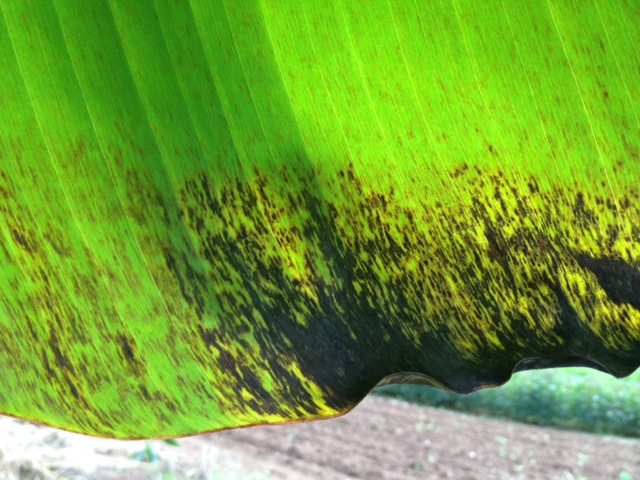
\includegraphics[width=.8\linewidth]{Roya_a}
  \caption{}
  \label{fig:sfig1}
\end{subfigure}
\begin{subfigure}{.3\textwidth}
  \centering
  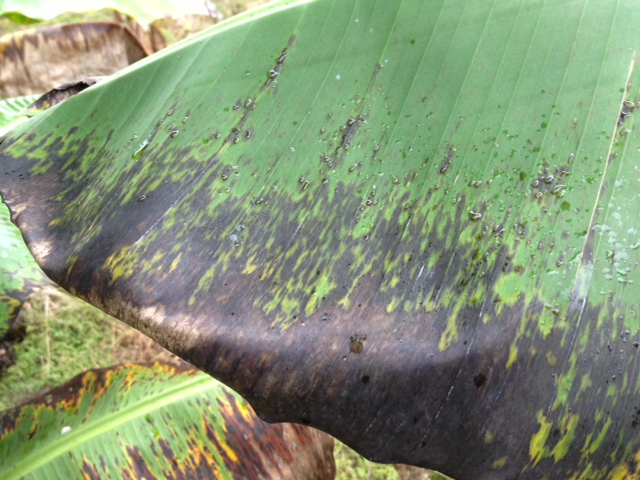
\includegraphics[width=.8\linewidth]{Roya_b}
  \caption{}
  \label{fig:sfig2}
\end{subfigure}
\begin{subfigure}{.3\textwidth}
  \centering
  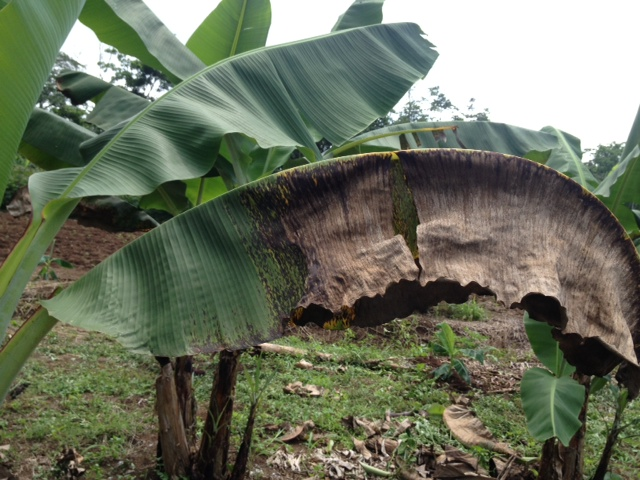
\includegraphics[width=.8\linewidth]{Roya_c}
  \caption{}
  \label{fig:sfig3}
\end{subfigure}
\caption{Examples of three disease stages of the black Sigatoka. (a) Initial stage. (b) Intermediate stage, and (c) Advanced stage.} 
\label{figura1} 
\end{figure}

According to studies by the National Banana Corporation of Costa Rica
(Corbana) made in 2013, considering on average between 53 thru 57
cycles of fungicide applications per farm, the cost per hectare per
year ranged between \$1800 USD and thru \$1900 USD. This represents
about 0.76 cents of the price of a box of 18.14 kilograms. Overall,
this represents 10\% to 12\% of the total production cost
\citet{Bresciani2015}.

The past and present disease development rate can in principle be used
to predict its future behavior, tendencies and to determine whether
particular fungicide spray schedules will be able to effectively and
economically control the disease \citet{ChuangJeger1987}.

There are efforts to apply machine learning methods for
decision-making in agriculture, including the control of crop
diseases. For example, \cite{Camargo2012} present an intelligent
systems for the assessment of crop disorders, \cite{Huang2010}
introduce a plant virus identification method based on neural networks
with an evolutionary preprocessing stage, \cite{Kim2014} summarize in
their survey crop pests prediction methods using regression and
machine learning approaches, while \cite{Zhao2013} present an
intelligent agricultural forecasting system based on wireless sensor
networks.

In this work, we compare four machine learning methods: support vector
regression (SVR), echo state networks (ESN), ridge regression, and
ordinary least squares linear regression, to predict the black
Sigatoka disease development rate.

The main contribution of this work is a comparison between machine
learning methods to forecast black Sigatoka development rate.


\section{Materials and methods}

\subsection{Concepts}

\subsubsection{Biological warning system}

The system measures the disease development state to determine when to
apply fungicides \citep{MarinVargas1995}.  This system is based on two
components: a climate component, which is given by the Piche
evaporation and a biological component, given by the stage of progress
or the rate of disease development. Originally, this system was
designed to work with young plants. One selected plant must exhibit a
normal growth and be in a place that enforces a healthy
development. The plant must start with 5 to 6 true leaves. The
assessments are made at fixed intervals of seven days as long as
possible, on the same plant. The first observations should consider
the leaf emission, also the level of infection on the leaves should be
evaluated considering the stages of development
\citep{MarinVargas1995}.

\subsubsection{Support Vector Regression (SVR)}
From the perspective of Support Vector Regression (SVR) the regression function $y = f(s)$ for a given dataset $D ={(s_i,y_i ) }_(i=1)^n$ , is represented as a linear function of the form (Wei, Tao, ZhuoShu, and Zio, 2013):
$f(s)=w^T s+b$
where 	$w$ and $b$ are respectively the weight vector and the intercept of the model, and they are selected to find an optimal fit to the data available in $D$.
For nonlinear cases, one proceeds by mapping the input p-dimensional vectors via a nonlinear function $ɸ∶R^p→F$, onto the feature space F.  After nonlinear mapping, the regression function evolves to a pervasive form:
$f(s)=w^T ɸ(s)+b$
SVR uses the є-insensitive loss function:
$l=|y-f(s)|_є= {█(0,   |y-f(s)|_  ≤ є@|y-f(s)|_ - є,     else)┤$
which ignores the error if the difference between the prediction value and the actual value is smaller than $є$.
$є-insensitive loss function$ allows to find the coefficients $w$ and $b$ by solving a convex optimization problem, which balances the empirical error and the generalization ability. In SVR, the empirical error is measured by the loss function є-insensitive and the generalization ability is measured by the Euclidean norm of $w$. Then, the optimization problem to identify the regression model can be formulated by (Wei, Tao, ZhuoShu, and Zio, 2013):
$minimize    J(w,ξ_i,ξ_i^* )=  1/2  ||w| |^2+ C ∑_(i=1)^n▒〖(ξ_i,ξ_i^*)〗
subject to 	{█(y_i- w^T  ɸ(s)-b  ≤   є+ξ_i@w^T  ɸ(s)+b- y_i   ≤   є+ξ_i^*     i=1,…,n@ξ_i,ξ_i^(* )≥0)┤$
where C denotes the penalty parameter between empirical and generalization errors, and  $ξ_i,ξ_i^(* )$are slack variables, as shown in Fig 2.
 
Fig 2: є-insensitive loss function (Wei, Tao, ZhuoShu, and Zio, 2013)
The solution of this optimization problem by the Lagrange method is:
$f(s)=w^T ɸ(s)+b= ∑_(i=1)^n▒〖(α_i-α_i^* )K(s,s_i )+b〗$
where $α_i,α_i^*$  are the Lagrange multipliers of the optimization problem’s dual form and $K(s_i,s_j )$ is the kernel function satisfying Mercer condition, and can be described by:
$K(s_i,s_j )=〈ɸ(s_i )  ɸ(s_j)〉  $
Common kernel functions are: linear, polynomial and sigmoid.
Operations in the kernel function K(s,s_i ) are performed in the input space rather than in the potentially high dimensional feature space of ɸ. An inner product in the feature space has an equivalent kernel in the input space (Alonso, Rodríguez Castañón, and Bahamonde, 2013).

\subsubsection{Ordinary least square}
This method fits a linear model with coefficients w = (w1,...,wp) to minimize the residual sum of squares between the observed responses in the dataset, and the responses predicted by the linear approximation. Mathematically it solves a problem of the form (scikit-learn developer, 2014):
〖■(min@w) 〗⁡〖‖Xw-y‖_2^2 〗

\subsubsection{Ridge regression}

This addresses some of the problems of Ordinary Least Squares by imposing a penalty on the size of coefficients. The ridge coefficients minimize a penalized residual sum of squares (scikit-learn developer, 2014):
〖■(min@w) 〗⁡〖‖Xw-y‖_2^2 〗+ α‖w‖_2^2
Here, α ˃ 0 is a complexity parameter that controls the amount of shrinkage: the larger the value of α, the greater the amount of shrinkage and thus the coefficients become more robust to collinearity.
\subsubsection{Echo State Networks (ESN)}
Recurrent Neural Networks (RNN) are useful for temporal patterns, but when they are trained with backpropagation method, they are very slow.  Echo State Network (ESN) is an alternative training method to solve that problem.  ESN is based on the observation that if a random RNN possesses certain algebraic properties, training only a linear readout from it is often sufficient to achieve excellent performance in practical applications (Lukoševičius and Jaeger, 2009). 
For a given training input signal u(n)  ϵ R^(N_u ) a desired target output signal y^(target(n))  ϵ R^(N_y )
is known. Here n = 1, . . . ,T is the discrete time and T is the number of data points in the training dataset. The task is to learn a model with output y(n)  ϵ R^(N_y ), where y(n) matches y^target(n) (n) as well as possible, minimizing an error measure E(y,y^target), and, more importantly, generalizes well to unseen data. The untrained RNN part of an ESN is called a dynamical reservoir, and the resulting states x(n) are termed echoes of its input history
 (Lukoševičius M. , 2012). Finally, these signals are sent to an output layer as shown in the following Fig.
 
Figure 3: An echo state network (Lukosevicius, 2012)
The connections between the different elements of an Echo State Network have weights randomly generated. The weights of the internal connections of the reservoir (W) as well as the weights of the input layer (Win), after being generated are set statically during all stages of implementation of the algorithm. The weights between the reservoir and the output layer (Wout) are subject to changes of a supervised learning algorithm to correct the degree of error generated by the entire system (Lukoševičius M. , 2012).
Related works
A related work, no machine learning approach, was performed by Romero (1995) who in the third chapter of his doctoral thesis in the field of plant pathology, proposed regression models using stepwise procedure to predict incubation and latency times of black Sigatoka. The author performed experiments on two farms located in Costa Rica (Rita and Waldeck, the same as those used in this study but with different names). The time intervals used for that study were: December 1993 thru August 1995. Romero concluded that the model to predict the incubation period accounted a R2 of 69\% in his observed data but it was not a good predictor when it was validated against an independent dataset (cross validation). For latency, he developed two models that accounted a R2 of 78\% in the observed data, however, when validated against an independent dataset (cross validation), the model was incorrect for Weldeck, and for Rita obtained an adjusted R2 of 82\%. 
A machine learning method was proposed by Glezakos, Moschopoulou, Tsiligiridis, Kintzios, and Yialouris (2010), who presented a genetic algorithm as to smooth out the initial information while, the so produced meta-data sets were used in the training and testing of the applied neural network, producing fitter training data. Given the features of the acquired virus time-series signals of the problem under study, an evolutionary method was proposed in order to produce meta-data from the original time-series initial information, reduce the dimensionality of the input data space, and eliminating the noise inherent in the initial raw information The method was tested against some of the most commonly used classifiers in machine learning (Bayes, Trees and k-NN) via cross-validation and proved its potential towards assisting virus identification. They made their test with CGMM and TR viruses.
In agricultural area, Alves, de Carvalho, Pozza, Sanches, and Mai (2011) selected the zones that are potentially favorable to coffee, soybean and banana diseases in Brazil according to the spatial-temporal variability of climatic variables and the geographical distribution of hosts. Their study applied methodology enabled the visualization of the variation of areas favorable to epidemics under future scenarios of climate change. The geoscientific and statistical modeling techniques developed in that study enabled the development of predictive models and the characterization of risk areas for soybean rust, coffee rust and black Sigatoka disease of banana.
There have been attempts to generate software tools, Camargo, Molina, Cadena-Torres, Jiménez, and Kim (2012) presented an information system for the assessment of plant disorders (Isacrodi). They proposed that experts will attain a much better accuracy than the Isacrodi classifier, particularly when provided with samples from the affected crop. However, where such expertise is not available, they suggest that Isacrodi can provide valuable support to farmers. Isacordi includes 15 crop disorders, but the black Sigatoka no is one. The prediction process is based on multi-class Support Vector Machines.
Regarding black Sigatoka with machine learning methods, Bendini, Moraes, da Silva, Tezuka, and Cruvinel (2013) presented a study about the risk analysis of black Sigatoka occurrence based on polynomial models. A case study was developed in a commercial banana plantation located in Jacupiranga, Brazil, it was monitored weekly during the period from February to December 2005. Data were the weekly monitoring of the disease’s evolution stage, time series of meteorological data and remote sensing data. They obtained a model to estimate the evolution of the disease from satellite imagery. This model relates gray levels (NC) of the corresponding image, band 2 of the Landsat-5 satellite, with the progress status or disease severity (EE): Authors express have reach an R2 of 90%.
Also there are research related to banana fruit, Soares, Pasqual, Lacerda, Silva, and Donato (2014) show in their study that  to the analyses, the neural network proved to be more accurate in forecasting the weight of the bunch in comparison to the multiple linear regressions in terms of the mean prediction-error (MPE = 1.40), mean square deviation (MSD = 2.29) and coefficient of determination (R2 = 91%).
In general, machine learning methods applied to prediction plant diseases can be classified in two main approaches: 1) Those that their main inputs are images, and 2) Those that their main inputs are environmental and biological variables. Our study is focus in the second one.

\subsubsection{Data}
In this work we used data acquired in two research farms of Corbana in Costa Rica: 1) 28 Millas (located at Matina) and La Rita (located at Pococí), both in the province of Limón, Costa Rica. The banana type is Musa AAA, subgroup Cavendish, cv. Grande Naine. Table 1 shows the variables considered initially.
Table 1 Variables used in the study
Variable	Meaning
T_(a_max )	Max air temperature
T_(a_min )	Min air temperature
T ̅_a	Mean air temperature
H	Humidity
H_min	Min humidity
H_max	Max humidity
R	Solar radiation
P ̅	Mean precipitation
W_max	Max speed wind
W ̅	Mean speed wind
L_2	Biological warning system – Leaf 2
L_3	Biological warning system – Leaf 3
L_4	Biological warning system – Leaf 4
ES	Biological warning system – Evolution Stage
The value to be predicted in all cases was ES, that is the total measure of the biological warning system.
The data on the biological warning system are collected once a week. Although Corbana has meteorological stations that take data every five minutes, for these experiments, weekly averages generated by nearby stations to each of the farms were used.
The time intervals used for this study were: La Rita, week 48 of 2002 to week 17 of the 2015 (647 weeks) and for 28 Miles, week 37 of 2003 to week 18 of 2015 (605 weeks).
Data preprocessing
In 28 Miles farm we detect that 1\% of the data were missing, while in La Rita 2.25\% of the data were missing. To complete the missing value we use spline interpolation. The data collected did not exhibit outliers.
Due the fact that the variables measure meteorological or biological process, they are discretized in order to reflect trends in the data rather than the specific continuous values. The coefficient of variation C_v (x) of each variable x was used to determine the numbers of discretizations with:
n= ⌊100 C_v (x)⌋
Each discretization range was uniformly partitioned. Besides enabling the capture of tendencies, the discretization removes the effect of small variations in the data collection, either by inaccuracies of the instruments (meteorological variables) or by subjective bias introduced by the human who collects the data (biological warning system).
Each feature was scaled in a range 0 between 1. The variable to be predicted was not scaled.

\subsubsection{Evaluation criteria}

Although there are many types of indicators to assess the quality of the prediction, we selected the root mean square error (RMSE) and the determination coefficient (R2).  This decision is supported by the widespread use in machine learning and agriculture areas (Soares, Pasqual and Lacerda (2013); Soares, Pasqual and Lacerda (2014); Ibrahim and Wibowo (2014) and Demir and Bruzzone (2014)).  

\subsubsection{Methods}
This research had two phases.
{\bf Phase one } 

In the phase one, we did ten-fold-cross-validation and did a lot of proofs with different machine learning methods and different configuration. 
We proved with several combinations:
	Patterns: From one week of observed data to predict the next week until nine weeks before to predict two weeks later.
	Algorithms: Support vector regression with different kernel functions: linear, RBF (Gaussian) and sigmoid; echo state networks; ordinary least squares linear regression and ridge regression.
	Variables included in the model. We proved the following combinations:
	All variables.
	Only variables that according to expert judgment have more impact on the black Sigatoka development: humidity, precipitation, temperature and wind speed (Marin Vargas and Romero Calderón, 1995).
	From the four variables listed in the previous paragraph, runs were conducted using each of the variables separately, and combining other runs all the possible pairs of those four variables.
Phase two
In the second phase, we used the best configurations obtained en la phase one and did validation with the last 52 and 102 weeks. 
This second phase pretended to show how these methods behaved on a time of important climate change how are 2014 and 2015 years.
Programming environment
We use python programming language with the Integrated Development Environment (IDE) Spyder, particularly with libraries: pandas (Comunity, 2014); numpy (numpy.org, 2013); for SVR, ridge and ordinary least squares, we used sklearn (Pedregosa, et al., 2011); and for ESN the python-based code used belongs to Dr. Mantas Lukoševičius (2012) from which we made the necessary adjustments for the experiments of this research. The computer was a Lenovo ThinkPad, processor Intel(R) Core™ i7-4800MQ CPU @ 2.70GHz, 16.0 GB RAM, running Windows 8 Pro.






\section{Results}

\section{Discussion and conclusions}

\section{References}

\begin{thebibliography}{1}

\bibitem[Brescani, 2015]{Bresciani2015} Brescani, XXXXX.

\bibitem[Camargo et al.,2012]{Camargo2012} Camargo, A., Molina, J., Cadena-Torres, J., Jim\'enez, N., Kim, J. 2012. Intelligent systems for the assessment of crop disorders. Computers and Electronics in Agriculture(85), 1-7. doi:10.1016/j.compag.2012.02.017.

\bibitem[Chuang and Jeger, 1987]{ChuangJeger1987} Chuang, T., Jeger, M. 1987. Predicting the Rate of Development of Black Sigatoka ( Mycosphaerella fijiensis var. difformis ) Disease in Southern Taiwan. Phytopathology, 77, 1542-1547.

\bibitem[Huang et al., 2010]{Huang2010} Huang, Y., Lan, Y., Thomson, S., Fang, A., Hoffmann, W., Lacey, R. 2010. Development of soft computing and applications in agricultural and biological engineering. Computers and Electronics in Agriculture,(71(2)), 107–127. doi:10.1016/j.compag.

\bibitem[Kim et al., 2014]{Kim2014} Kim, Y., Yoo, S., Gu, Y., Lim, J., Han, D.,  Baik, S. 2014. Crop Pests Prediction Method Using Regression and Machine Learning Technology: Survey. IERI Procedia(6), 52–56. doi:10.1016/j.ieri.2014.03.009.

\bibitem[Marin and Romero, 1995]{MarinVargas1995} Marin Vargas, D., Romero Calderón, R. 1995. El combate de la Sigatoka Negra. Bolet\'in Departamento de Investigaciones, Corbana Costa Rica.

\bibitem[Zhao et al., 2013]{Zhao2013}Zhao, L., He, L., Harry, W., Jin, X. 2013. Intelligent Agricultural Forecasting System Based on Wireless Sensor. Journal of Networks(8), 1817–1824. doi:10.4304/jnw.8.8.1817-1824.

\end{thebibliography}

\end{document}